Motion is a simple concept representing playback state (media clock), as well
as functions for accessing and manipulating this state (media controls). As
such, similar constructs are found in most multimedia frameworks.

\begin{figure}[h]
%\sidecaption
\centering
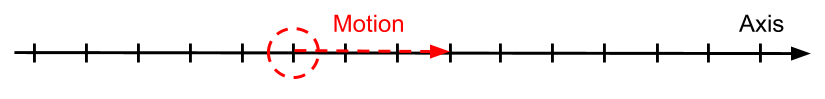
\includegraphics[scale=.4]{fig/motion-axis.png}
\caption{Motion: point moving along an axis. The current position
is marked with a red circle (dashed), and forward velocity of 3 units per second is
indicated by the red arrow (dashed).}
\label{fig:motion}
\end{figure}

As illustrated in Fig.~\ref{fig:motion}, motion represents movement (in real-
time) of a point, along an axis (timeline). At any moment the point has well
defined position, velocity and acceleration\footnote{Some animation frameworks
support acceleration. Acceleration broadens the utility of motions, yet will
likely be ignored in common use cases in classical media (see
Sect.~\ref{sec:toomuch}).}. Velocity and acceleration describe continuous
movements. Velocity is defined as position-change per second, whereas
acceleration is defined as position- change per second squared. Discrete jumps
on the timeline are also supported, simply by modifying the position of the
motion. A discrete jump from position A to C implies that the transition took
no time, and that no position B (between A and C) was visited. Not moving
(i.e. zero velocity and acceleration) is a special case of movement.

\runinhead{Internal State.}
\label{sec:internalstate}
Motion is defined by an internal clock and a vector (position, velocity,
acceleration, timestamp). The vector describes the initial state of the
current movement, timestamped relative to the internal clock. This way, future
states of the motion may be calculated precisely from the initial vector and
elapsed time. Furthermore, application programmers may control the motion
simply by supplying a new initial vector. The motion concept was first
published under the name Media State Vector (MSV)~\cite{msv}.


\subsection{Motion API}
\label{sec:motionapi}


Motions may constructed with a URL to an online motion. If the URL is omitted,
a purely local motion is created instead. 
\begin{lstlisting}[caption=Constructing a motion.]
var URL = "...";
var motion = new Motion(URL);
\end{lstlisting}

The \emph{Motion API} defines two operations,
\emph{query} and \emph{update}, and emits one \emph{change} event.


\runinhead{query():} 

The query operation returns a vector representing the current state of the
motion. This vector includes position, velocity and acceleration, as well as a
timestamp. For instance, if a query returns position 4.0 and velocity 1.0 and no acceleration, a
new query one second later will return position 5.0.

\begin{lstlisting}[caption=Querying the motion to get a snapshot vector.]
var v = motion.query();
console.log("pos:" + v.position);
console.log("vel:" + v.velocity);
console.log("acc:" + v.acceleration);
\end{lstlisting}


\runinhead{update(vector):} 

The update operation accepts a vector parameter specifying new values for
position, velocity and acceleration. This initiates a new movement for the
motion. Omitting say position implies that the current position will be used.
So, an update with velocity 0 pauses the motion at the current position.

\begin{lstlisting}[caption=Querying the motion for a snapshot vector.]
// play, resume
motion.update({ velocity: 1.0 }); 
// pause
motion.update({ velocity: 0.0 });
// jump and play from 10
motion.update({ position: 10.0, velocity: 1.0});
// jump to position 10, keeping the current velocity
motion.update({ position: 10.0 });
\end{lstlisting}


\runinhead{change event:}

Whenever the motion is updated, all event listeners (i.e. media components)
will immediately be invoked. Note that the change event is not emitted
periodically like the \emph{timeupdate} event of HTML5 media elements. The change event signifies the start of a
new movement, not the continuation of a movement.

\begin{lstlisting}[caption=Querying the motion for a snapshot vector.]
motion.on("change", function (e) {
  var v = motion.query();
  if (v.velocity === 0.0 && v.acceleration === 0.0) {
    console.log("I'm not moving!");
  } else {
    console.log("I'm moving!");
  }
});
\end{lstlisting}


\subsection{Programming with motions}

\runinhead{Online Motion:}

The Motion API is particularly designed to mediate access to online motions.
As discussed in Sect.~\ref{sec:model}, update operations are forwarded to the
online motion, and will not take effect until notification is received from
the online motion, and change events are emitted. In contrast, query is a local
(and cheap) operation. This ensures that media components may sample the
motion frequently if needed. In short, through the Motion API, online motions
are made available to Web developers as local objects. Only the latency of the
update operation is evidence of a distributed nature.

\runinhead{Using motions:}

Motions are resources used by Web applications, and the developer may define
as many as required. What purposes they serve in the application is up to the
programmer. If the motion should represent media offset in milliseconds, just
set the velocity to 1000 (advances the position of the motion by 1000
milliseconds per second). Or, for certain musical applications it may be
practical to let the motion represent beats per second. Note also that motion
may represent progress for different kinds of media. For instance, slides in a
slideshow or pages in a book. If a dataset is indexed by, say, height above
sea level, a motion could be used to animate how this data changes as you move
vertically, upwards or downwards.

\runinhead{Motion converters:}

A common challenge in media synchronization is that different sources of media
content may reference different timelines. For instance, one media stream may
have a logical timeline starting with 0, whereas another is timestamped with
epoch values. If the relation between these timelines is known (i.e. \emph{relative
skew}), it may be practical to create a skewed motion for one of the media
components, connected to the other motion. This is supported by \emph{motion
converters}. Multiple motion converters may be connected to a root motion, each
implementing different transformations such as scaling and looping. Motion
converters may also be chained. Motion converters implement the \emph{Motion API},
so media components can not distinguish between a motion and a motion
converter. Motion converters are implemented under the name \emph{timing converters}
in the Timingsrc programming model~\cite{timingsrc}.

\runinhead{Too much flexibility:}
\label{sec:toomuch}

The mathematical nature of the motion concept makes it flexible, yet for a
particular media component some of this flexibility may be unnecessary, or
even unwanted. For instance, the HTML5 media player will typically not be able
to operate well with negative velocities, very high velocities, or with
acceleration. Fortunately, it does not have to. Instead, the media player may
define alternative modes of operation as long as the motion is in an
unsupported state. It could show a still image every second for high velocity,
or simply stop operation altogether (e.g. black screen with error message).
Later, when motion re-enters a supported state, normal operation may be
resumed for the media player.

%\subsection {Summary}
%Motion is a simple concept encapsulating media clock and media controls. It is
%designed particularly to be monitored by multiple media components, and as an
%interface towards online motions.
